% !TeX spellcheck = en_US
\documentclass{pasa}

\title[Kuzushiji Recognition]{Kuzushiji Recognition \\ \large Cognitive Services 2018-19 project report}

\author[Matteo Rizzo, Alessandro Zangari]{\textbf{Matteo Rizzo} ~~~~~~~~~~~~~id. 1206694\\ \textbf{Alessandro Zangari} ~~~~id. 1207247\\}%
\date{September 2019}

% UNCOMMENT THE LINES BELOW IF YOU WISH TO USE BIBTEX
\usepackage[backend=biber,bibencoding=utf8,style=numeric-comp,maxcitenames=2,hyperref,backref]{biblatex}
%Citations may be made using the natbib commands \citet{},\citep{} etc.
%\usepackage[authoryear,backend=biber]{natbib}
%\bibpunct{(}{)}{;}{a}{}{,}
%\setlength{\bibsep}{0.3mm}

\usepackage[utf8]{inputenc}             % codifica di input; anche 
\usepackage[english]{babel}
\usepackage{aas_macros}
\usepackage[table,xcdraw]{xcolor}
\usepackage{dblfloatfix}
\usepackage{multirow}
\usepackage{hyperref} 
\hypersetup{
	colorlinks,
	citecolor=green,
	linkcolor=blue,
	urlcolor=blue,
	breaklinks=true,
	pdftitle={Kuzushiji Recognition - Cognitive Services 2018-19 project report},
	pdfauthor={Alessandro Zangari, Matteo Rizzo},
	pdfsubject={Text recognition of ancient Japanese characters},
	pdfkeywords={Kuzushiji, object detection, text recognition},
	pdfcreator={pdfLaTeX},
	pdfproducer={LaTeX}}
\usepackage{graphicx}
\graphicspath{{images/}}
\bibliography{bibliography.bib}


\begin{document}

% !TeX spellcheck = en_US
\begin{abstract}
	Automatic translation, natural language processing and other language related tasks are among the most challenging problems in computational linguistics. The ability of a machine to understand written and spoken language led to notable improvements in tasks such as documents digitization, speech synthesis and text mining, but text recognition in handwritten documents is still one of the most difficult task to deal with. However, the further improvements on deep neural networks for object recognition have definitely amended the performance in this area of research. Convolutional Neural Networks (CNN) and Recurrent Neural Networks (RCNN) in particular have been successfully applied to linguistic and vision tasks. Their ability to learn complex, non linear functions has been proven ideal to deal with the overwhelming number of features concealed in images and the complexity of languages. In this report, we show a deep-learning-based solution to the task proposed in the Kaggle competition “Kuzushiji Recognition”. The goal of the competition is translating ancient cursive handwritten Kuzushiji pages into modern Japanese. More precisely, a great number of different possible characters must be automatically detected and classified. Our approach is focused on a region-based model which uses a CenterNet like neural network to detect characters and then translates them into modern Japanese using a simple CNN. It resulted in 0.77 IoU score in detection, 0.94 accuracy of classification and a 0.797 modified $F_1$ score for the competition.
\end{abstract}


\begin{keywords}
	kuzushiji - text recognition - object detection
\end{keywords}


\maketitle

% --- INTRODUCTION ---

% !TeX spellcheck = en_US
\section{INTRODUCTION}
\label{sec:intro}

Kuzushiji is a Japanese cursive writing style which has been used in Japan for over a thousand years, beginning in the 8th century. Over 3 millions books, on a diverse array of topics such as literature, science, mathematics and cooking are preserved today. However, the standardization of Japanese textbooks known as the “Elementary School Order” in 1900, removed Kuzushiji from regular school curriculum, as modern Japanese print became popular. As a result, most Japanese natives today cannot read books written or printed just 120 years ago, and today there are very few fluent readers of Kuzushiji (only 0.01\% of modern Japanese natives) \cite{aboutkuz}. The objective of the project, inspired by a Kaggle competition promoted by the Center for Open Data in the Humanities \cite{competition}, is building an object detection system able to transcribe pages of ancient Kuzushiji handwritten documents into contemporary Japanese characters, as shown in figure \ref{fig:objective}. Due to the lack of available human resources, there has been a great deal of interest in using machine learning to automatically recognize these historical texts and transcribe them into modern Japanese characters. Nevertheless, several challenges in Kuzushiji recognition have made the performance of existing systems extremely poor. Our deep-learning-based approach achieved notable results, with 0.77 IoU score in detection, 0.94 accuracy of classification and a 0.797 modified $F_1$ score on the competition public test set.

\begin{figure}
	\centering
	\caption{A document written in Kuzushiji whose characters have been automatically translated into modern Japanese characters.}
	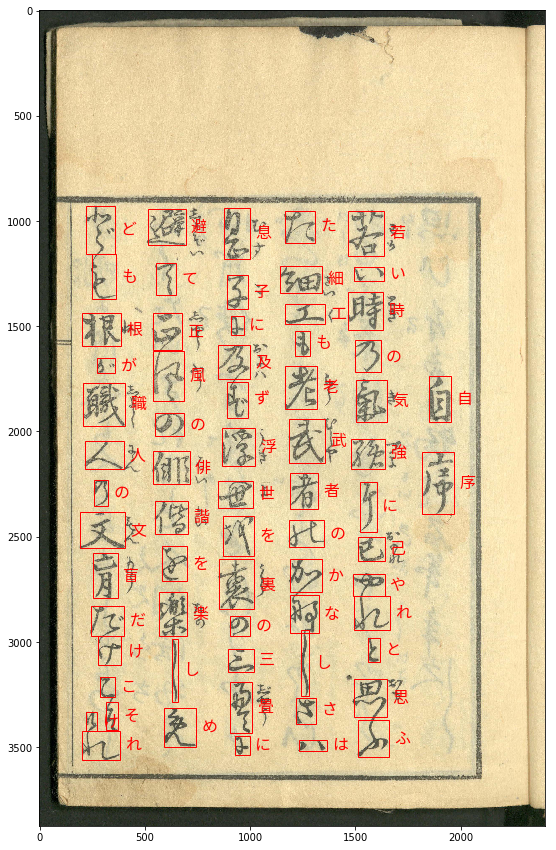
\includegraphics[width=0.6\columnwidth]{various/objective.png}
	\label{fig:objective}
\end{figure}

% --- RELATED WORK ---

\section{RELATED WORK}
\label{sec:relatedwork}

Optical Character Recognition (OCR) of cursive handwriting has proven to be a challenging problem. In particular, character segmentation is recognised as one of the major problems in recognizing unconstrained cursive characters or words. We can roughly divide the character recognition approaches into four categories:
\begin{enumerate}
	\item \textbf{Holistic approaches} (also called global approaches) try to avoid an explicit segmentation process, recognizing entire words without splitting them into single characters. This can be done using an end-to-end neural network and using heuristics based on the number of loops and vertical strokes in each text segment.
	\item \textbf{Classical approaches} perform character segmentation strictly before character classification and recognition, and the two steps are carried out independently. Our method belongs to this category.
	\item \textbf{Recognition-based segmentation approaches} interleaves character segmentation and character classification steps. This can be done by segmenting a word, then classify each character, and if the classifier confidence is not high enough repeat the segmentation step in a different way.
	\item \textbf{Mixed approaches} that combine various techniques belonging to the previous points.
\end{enumerate}

Various text detection algorithms have  been proposed in literature, and we present a selection of articles describing some of these algorithms, summing up the key points and results. Jo, Koo, Soh, Cho presented an end-to-end text segmentation approach to separate handwritten text from machine printed documents, like filled out forms and book side annotations. They use a Convolutional Neural Network (CNN) with an encoder-decoder architecture similar to U-Net, using max pooling as downsample operators in the encoder and transposed convolution for upsampling in the decoder. The network is trained end-to-end using Adam optimizer and focal loss, taking in consideration class imbalance. They report a 92.50\% detection accuracy, but state that this was significantly reduced when handwritten text overlapped with printed text.
Blumenstein proposes a three steps neural-based segmentation technique. The first step includes an improved heuristic to oversegment the text, that achieved high performances at detecting segmentation points under overlapping strokes. It features a modified vertical histogram analysis more suitable to distinguish between ligatures and holes (empty space inside a letter). The second step involves two neural networks trained with a set of features extracted from the over-segmented words that outputs a confidence score for every segmentation point. The last step consists into fusing the confidence values from the networks to obtain the final word segmentation. The experiments are conducted over a small dataset of cursive english words and resulted in a clear improvement of segmentation score with respect to the standard (non-enhanced) oversegmentation method.
Bluche, Louradour, Messina use an end-to-end method to recognise paragraphs of text taken from the IAM database, consisting of images of unconstrained handwritten english text documents. They use a Multi-Dimensional Long Short-Term Memory Recurrent Neural Network (MDLSTM-RCNN) to model an attention based mechanism, effectively reading characters in the right order and learning to skip images, noise and line breaks, emulating the attention mechanism of a human reader. They employ a MDLSTM encoder to produce a feature vector that is passed to the MDLSTM modelling the attention mechanism. The weighted sum of the encoder features and the attention weights are passed to a LSTM layer and to the multilayer perceptron that acts as a decoder. The experiments highlight the power of the proposed attention mechanism to recognise full lines of text, while the performances significantly decrease over single words or very short sentences.
Another interesting work with an attention based model applied specifically to Kuzushiji character recognition and translation was presented by Duc Le, Kitamoto, Clanuwat and featured an encoder-decoder architecture with a CNN for feature extraction and an LSTM decoder with an attention model for generating the target Japanese characters. The encoder CNN is a DenseNet which they claim to outperform ResNet and VGG for some recognition tasks. The experiments have been conducted on multiple tasks, from the translation of single characters, to the translation of entire sentences. Their system outperformed Faster R-CNN and VGG-encoded models based on the reported sentence error rate (SER) metric.
Finally, regarding the recognition of single japanese characters, Banerjee proposes a variation on a previous popular algorithm called STRICT-FB, that allows to extract a set of geometric and topological features that allows to overcome the difficulties in recognizing very similar hiragana characters. One of this features is the Center of Gravity (CoG), obtained from the number of black pixels and their relative positions inside an enclosing circle drawn around the character. The author reported an average recognition rate of 94.1\%, better than the results obtained with the original algorithm, conducted over a set of handwritten character with similar size.

% --- APPROACHES ---

% !TeX spellcheck = en_US
\section{APPROACHES}
\label{sec:approaches}

In general, the task of text detection consists of recognizing the required text from images. In some tasks, like ours, it is required to find all the fragments of text within a page, but for other purposes reading the entire document is not needed, rather the objective is extracting a piece of information within it (e.g. credit card number, amount and date from bills, etc). The main reason why this problem, and, in general, every object detection problem, can not be solved by a standard convolutional network followed by a fully connected layer is that, since the number of occurrences of objects (characters in our case) is not fixed, the length of the output layer is variable. A naive solution to this issue would be taking different regions of interest from the image and use a CNN to classify the objects within those regions. The problem with this approach is that the objects of interest might have different spatial locations within the image and different aspect ratios. Hence, a select over a huge number of regions would be needed, and this may not be computationally affordable. Therefore, a number of algorithms have been developed to balance computational costs and time without renouncing to good detection performances.

\subsection{Region-based}
\label{ssec:regionbased}

Region-based methods work by finding all the regions which may contain an object, and then passing those regions to a classifier which defines the locations of the required objects. In order to bypass the problem of selecting a huge number of regions, the R-CNN uses a method that implies a selective search to extract about 2000 regions from the image, which are called region proposals. These candidate regions are resized into square images and fed into a convolutional neural network that produces a 4096-dimensional feature vector as output. The CNN acts as a feature extractor and the extracted features are then fed into an SVM to classify the presence of the object within that candidate region proposal \cite{Gandhi2018}. A simplified overview of this approach is presented in figure \ref{fig:rcnn}.

\begin{figure}[h]
	\caption{Overview of the R-CNN object detection system \cite{Gandhi2018}.}
	\centering
	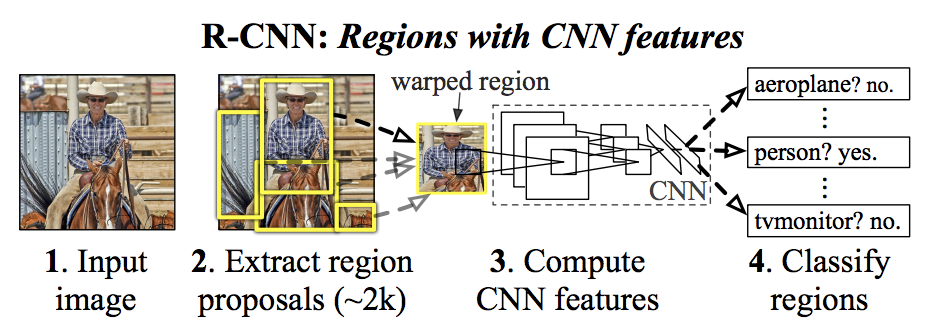
\includegraphics[width=0.5\textwidth]{approaches/RCNN.png}
	\label{fig:rcnn}
\end{figure}

Note that this approach is considered more accurate, but it is quite slow if compared with other methods. It takes a huge amount of time to train the network as the model needs to classify 2000 region proposals per image. Furthermore, the selective search algorithm is a fixed algorithm. Therefore, no learning is happening at that stage, which could lead to the generation of bad candidate region proposals. However, improvements have been shown in subsequent research. The Fast R-CNN algorithm solved some of the major drawbacks of R-CNN t	o build a faster object detection system: the approach is similar to the R-CNN algorithm, but instead of feeding the region proposals to the CNN, the whole input image is fed to the CNN to generate a convolutional feature map \cite{Girshick2015-ay}. The Faster R-CNN algorithm then eliminates the selective search algorithm and lets the network learn the region proposals by itself \cite{Ren2017-fu}.

\subsection{Single shot}
\label{ssec:singleshot}

Single shot detectors predict both the bounding box and the class of an object at the same time. Being a single step process, it is much faster and indicated for real-time object detection. Instead of having a network produce proposals, the single shot approach implies the exploitation of a set of predefined boxes to look for objects. In order to understand what is in an image, the input is fed through a standard convolutional network to build a rich feature representation of the original image. This part of the architecture is the "backbone" network, which is usually pre-trained as an image classifier to more cheaply learn how to extract features from an image. After pre-training the backbone architecture as an image classifier, its last few layers are removed, so that its output consists of a collection of stacked feature maps which describe the original image in a low spatial resolution but in a high feature (channel) resolution. In order to detect an object, another convolutional layer is added, and the kernel parameters must be learned, which combine the context of all the feature maps of the object in order to produce an activation corresponding with the grid cell which contains it \cite{Jordan2018}. This process is showed in figure \ref{fig:ssd}. \\

\begin{figure}[h]
	\caption{Combination of the feature maps to produce an activation in the grid cell responsible for detecting an object in a single shot detector \cite{Jordan2018}.}
	\centering
	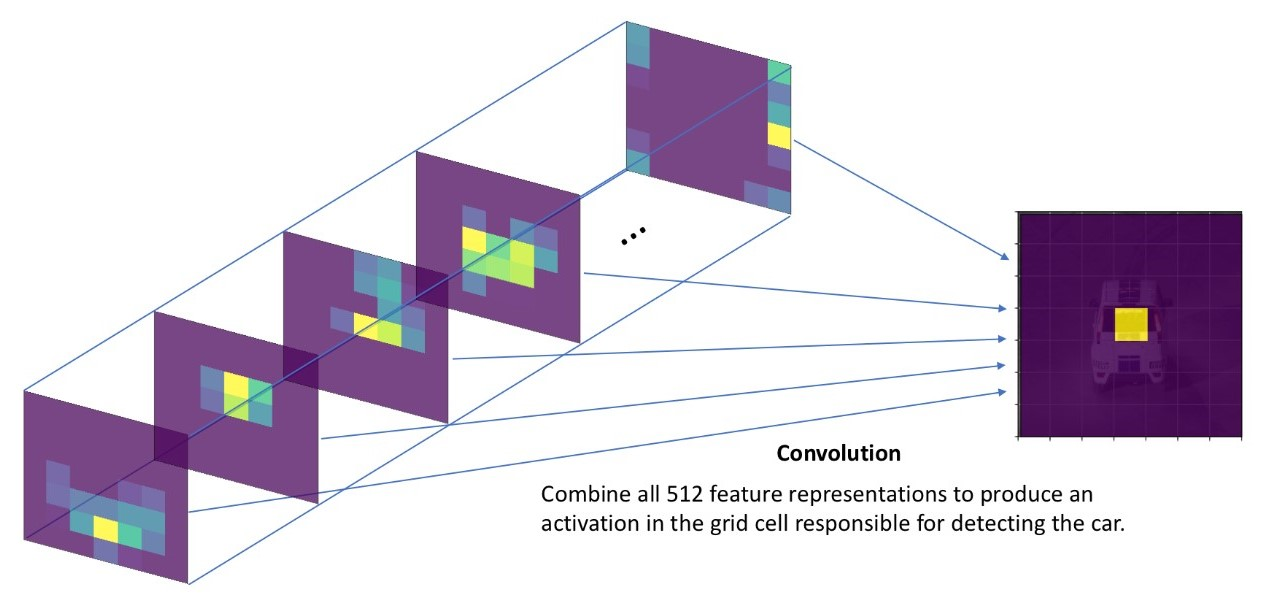
\includegraphics[width=0.5\textwidth]{approaches/SSD.jpg}
	\label{fig:ssd}
\end{figure}

Because of the convolutional nature of the detection process, multiple objects can be detected in parallel, substantially increasing the overall speed of the algorithm. However, the method also ends up predicting for a large number of grid cells where no object is found. Although the majority of the redundant bounding boxes could be filtered out by selecting a proper confidence threshold, multiple high-confidence predictions describing the same object may persist. Thus, a method is needed for removing redundant object predictions such that each object is described by a single bounding box. To accomplish this, a technique known as non-maximum suppression is used. At a high level, this technique will look at much overlapping bounding boxes and suppress all the predictions except the one with the highest confidence value. The strategy is outlined in figure \ref{fig:nms}.

\begin{figure}[h]
	\caption{Non-maximum suppression strategy \cite{Jordan2018}.}
	\centering
	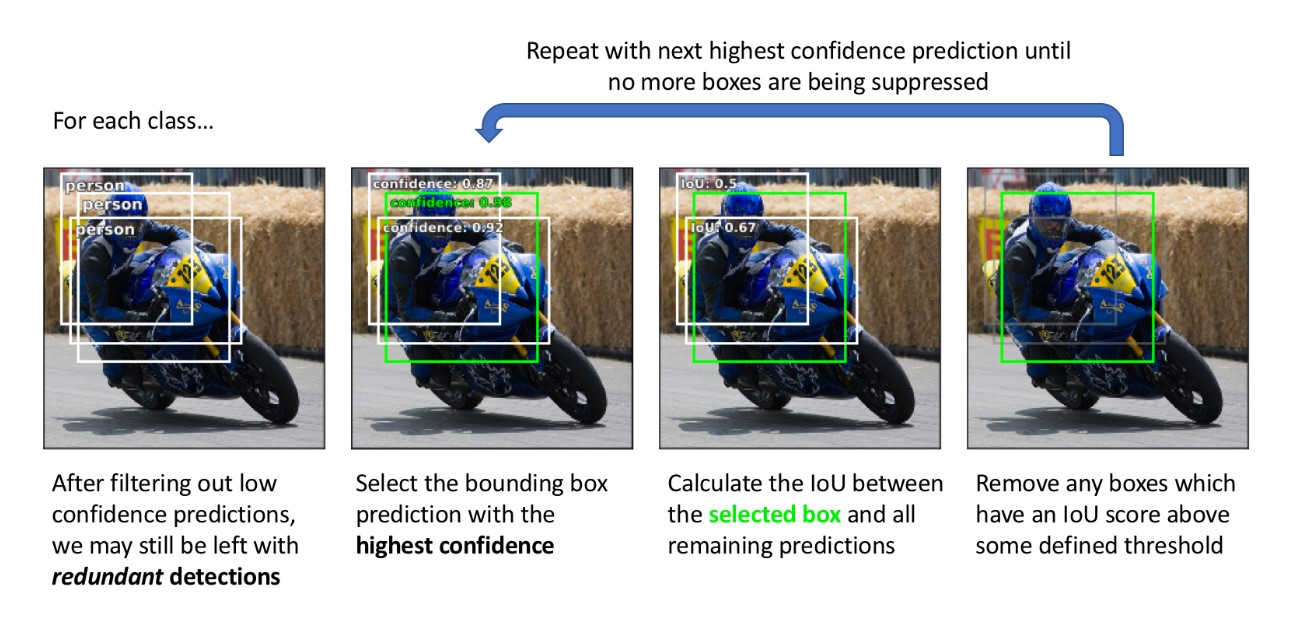
\includegraphics[width=0.5\textwidth]{approaches/nms.jpg}
	\label{fig:nms}
\end{figure}

One of the most popular Single Shot detectors is the YOLO (You Only Look Once) network. The original YOLO network (YOLO v1) \cite{Redmon2015-cy} uses a modified GoogLeNet as the backbone network. Later on, \citeauthor{Redmon2016-ad}\cite{Redmon2016-ad} proposed a new model named DarkNet-19 (YOLO v2) which follows the general design of $3\times3$ filters, doubling the number of channels at each pooling step; 1x1 filters are also used to periodically compress the feature representation throughout the network. Finally, in a different paper, \citeauthor{Redmon_undated-wa}\cite{Redmon_undated-wa} introduces a new, larger model named DarkNet-53 (YOLO v3) which offers improved performance over its predecessor. All of these models were first pre-trained as image classifiers before being adapted for the detection task, adapting the classification network for detection simply consists of removing the last few layers of the network and adding a convolutional layer with $B(5+C)$ filters to produce the NNB bounding box predictions. The first iteration of the YOLO model directly predicts all the four values which describe a bounding box. The x and y coordinates of each bounding box are defined relative to the top left corner of each grid cell and normalized by the cell dimensions such that the coordinate values are bounded between 0 and 1. The width and height of the boxes are user-defined, such that the model predicts the square-root width and height, and an L2 loss is applied during training. This formulation was later revised to introduce the concept of a bounding box prior: rather than expecting the model to directly produce unique bounding box descriptors for each new image, the user will define a collection of bounding boxes with varying aspect ratios which embed some prior information about the shape of objects that are to be expected in the examples. Rather than directly predicting the bounding box dimensions, the task is reformulated in order to simply predict the offset from the bounding box prior dimensions such that it is possible to fine-tune the predicted bounding box dimensions. This reformulation makes the prediction task easier to learn.

% --- DATASET ---

% !TeX spellcheck = en_US
\section{DATASET}
\label{sec:dataset}

The dataset provided by the hosts of the competition consists of a training set of 3881 high-resolution images, and a test set of 4150 high-resolution images. No other dataset  has been used. The labels are presented as the unicode encoding of the character to be recognized and the complete annotation (i.e. top, left, bottom, right) of the bounding box that encloses it. A standard image from the dataset is shown in figure \ref{fig:dataset_example}. \\

\begin{figure}[h]
	\caption{Example of standard image from the dataset.}
	\centering
	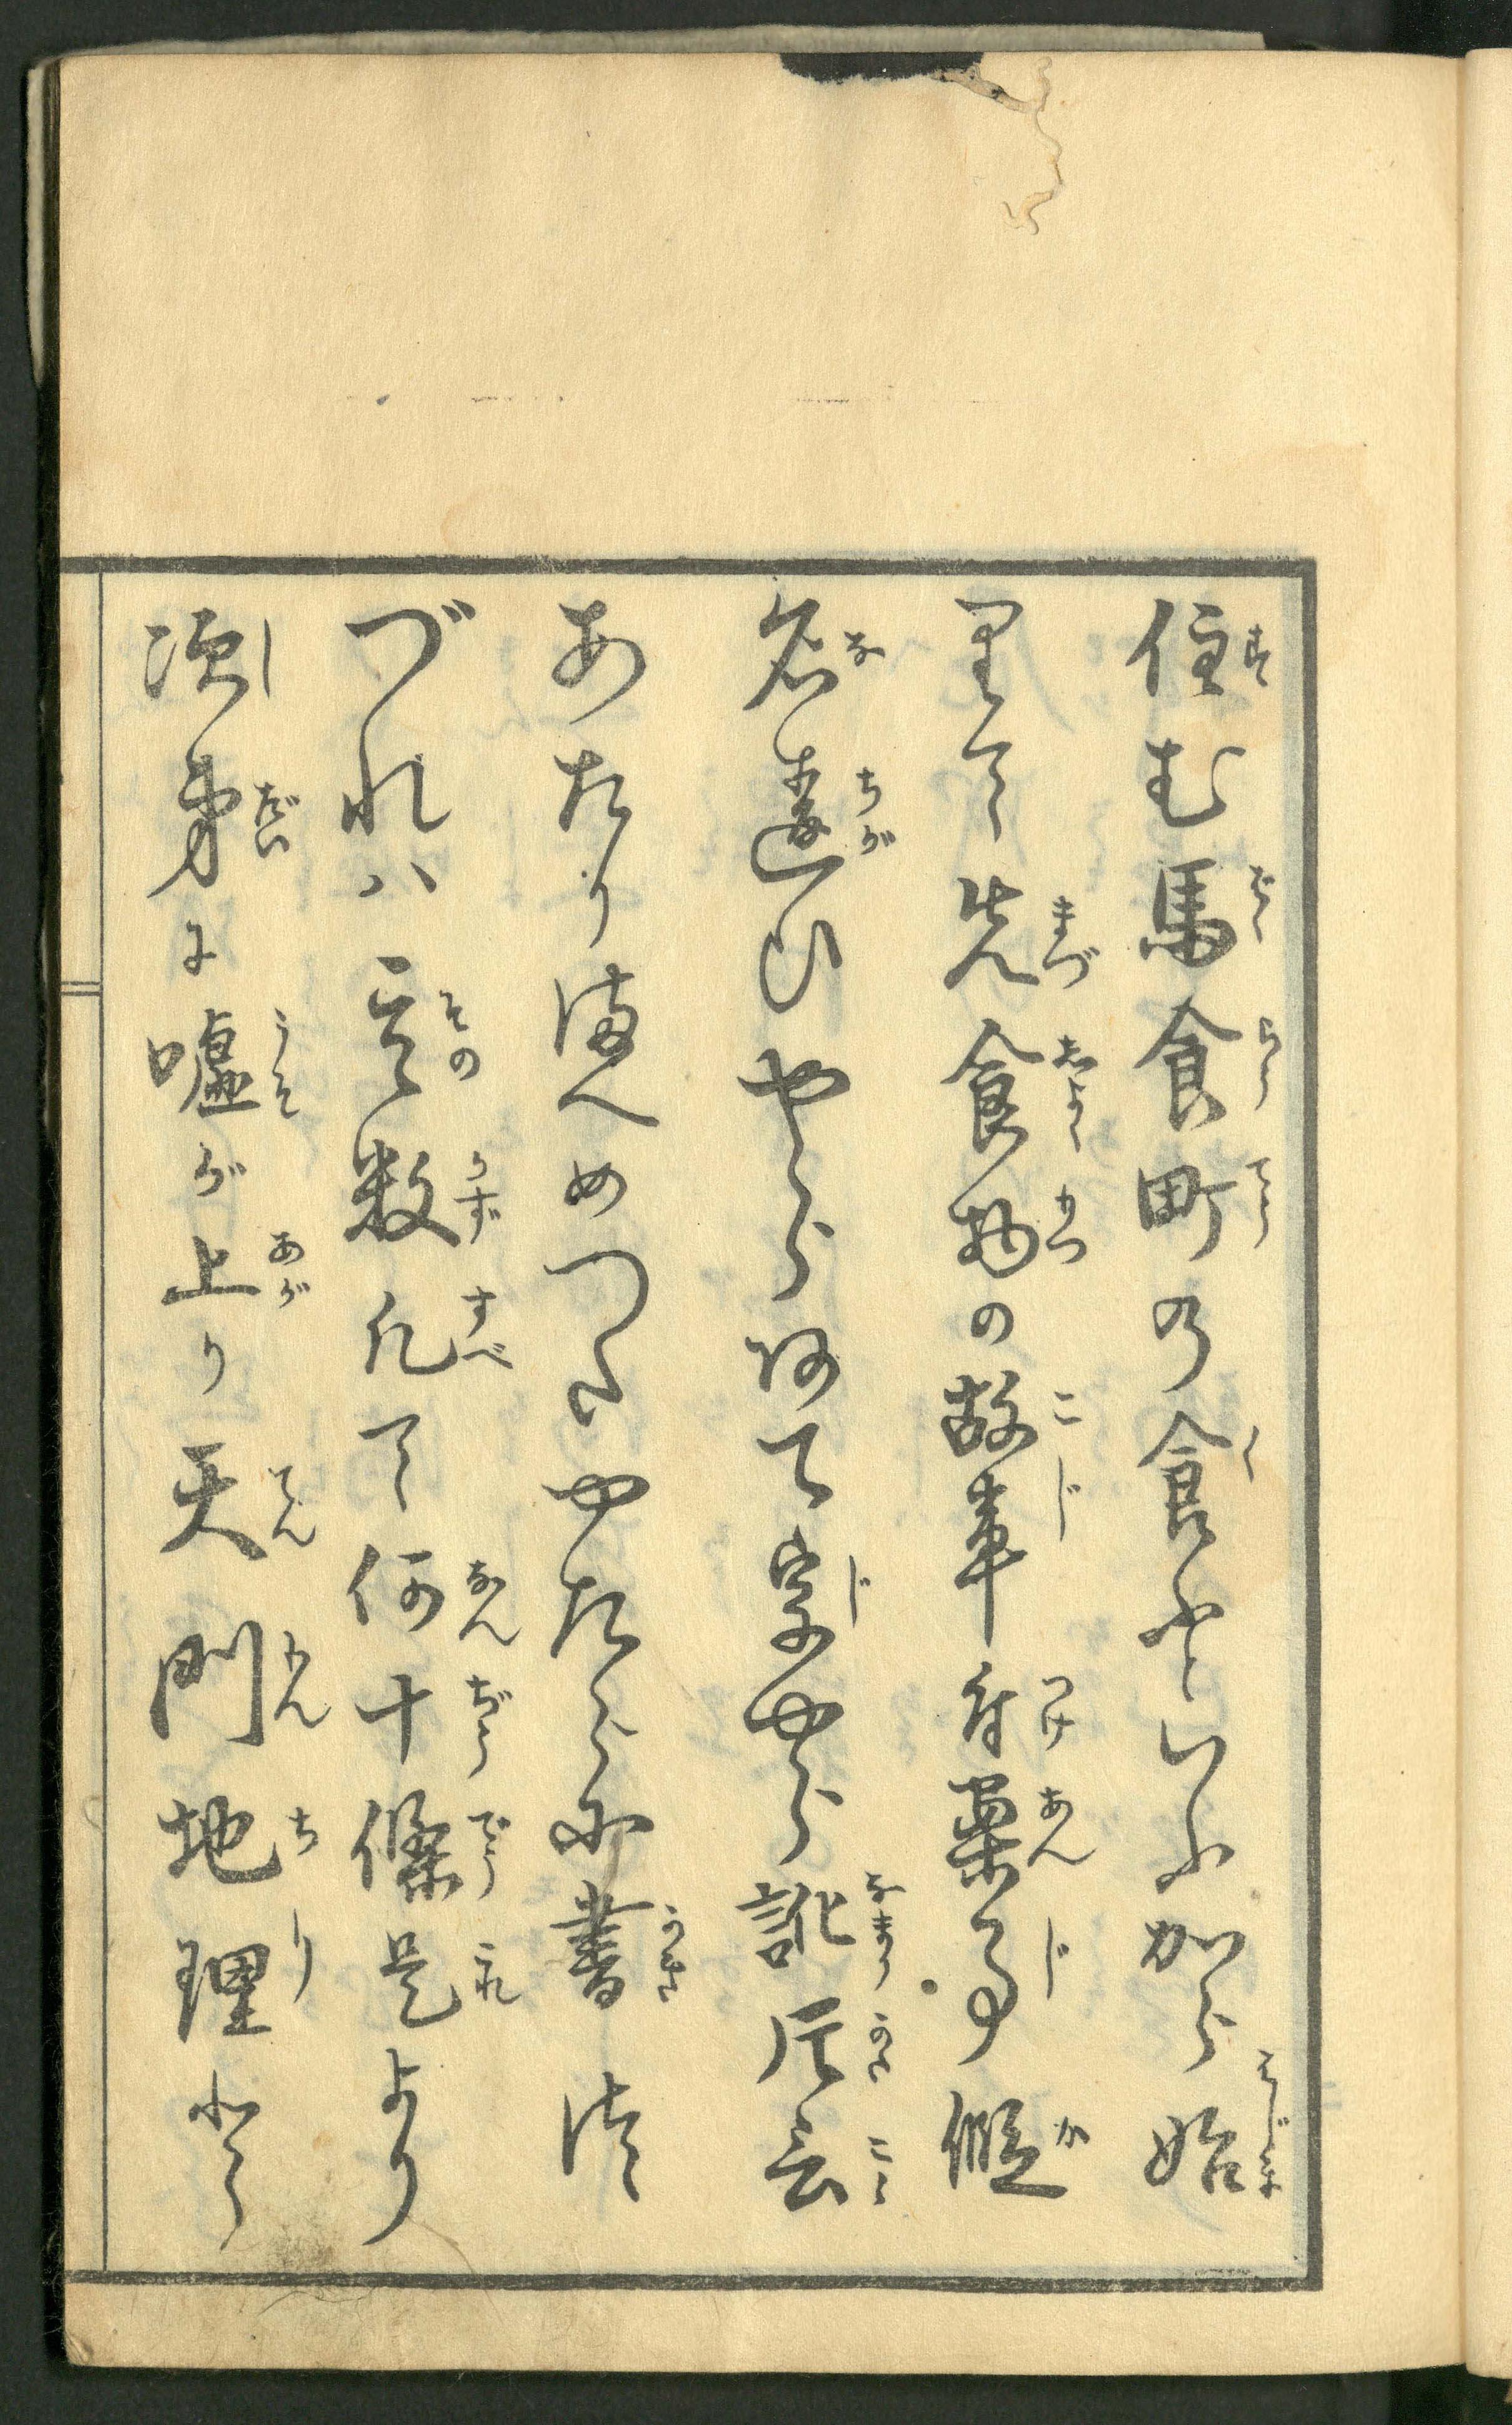
\includegraphics[width=0.3\textwidth]{dataset/dataset_example.jpg}
	\label{fig:dataset_example}
\end{figure}

Several peculiarities of Kuzushiji characters have made their automatic recognition notoriously challenging. Of course, being a cursive writing style, in many cases, characters are connected or overlapped. Furthermore, in Kuzushiji documents Kanji, Hiragana and Katakana, three very different kinds of Japanese writing, are all used, possibly in the same page. A peculiar characteristic of one of these kinds of writing, Classical Hiragana, is that many characters which can only be written in a single way in modern Japanese can be written in many different ways in Kuzushiji, generating multiple orthographic variations of the same character. Besides, a few characters in Kuzushiji also look very similar, making it quite hard to tell what character it is without considering the above character within the context, which may be an interesting hook for the application of a language model. However, the layout of Kuzushiji characters (while normally arranged into columns) does not follow a single simple rule, so it is not always trivial to express the characters as a sequence. The data analysis also brought out some interesting facts about the dataset. First of all, only 4212 out of the possible 4787 Kuzushiji characters are present within the training set. Despite the total number of unique characters in the dataset being quite high, the frequency distribution is very long-tailed and a large fraction of the characters (Kanji with very specific meaning) may only appear once or twice in a book. Therefore, the dataset is highly unbalanced. Some images also contain illustrations only, in which case no character should be detected. In a similar fashion, the thin paper of the manuscripts sometimes lets characters of the following page transpire. Those characters should be ignored and may score some false positives.


% --- METHOD ---

% !TeX spellcheck = en_US
\section{METHOD}
\label{sec:method}

For tackling the here proposed problem, a YOLO detector has been used at first. The YOLO network usually relies on Darknet, an open source neural network framework written in C and CUDA. However, we initially relied on a popular python translation of Darknet, called Darkflow, to set up the learning pipeline. Since Darkflow does not support YOLO v3 yet, we used YOLO v2 as the model to be fine-tuned for an initial testing. Anyway, this approach did not yield any good result, with the network not being able to properly converge. A variety of setups of parameters were tried, but the loss and moving average loss values never decreased under the approximate threshold of 30 (starting from about 130). In particular, the learning rate has ranged from $1 \cdot 10-3$ to $5 \cdot 10-7$ with a step of a 10 factor and fixed decay equal to $5 \cdot 10-4$, batch size has ranged from 1 to 64 with step 8, and both ‘Adam’ and ‘sgd’ optimizers have been tested. Moving to YOLO v3 using an open source Keras implementation resulted approximately in the same bad performance with the same setups. The training was performed both using and not using different weights pretrained on COCO dataset, namely those provided by Joseph Redmon via the official website of the YOLO project. In light of these results, a different approach has been preferred. Instead of using an end-to-end model to detect bounding boxes and translate each character, we pipelined two different models: 1) a model to detect the characters and 2) a model to predict the specific Japanese character from each detected object. In particular, we implemented a CenterNet architecture for detection and a quite simple CNN for classification. The name CenterNet is used because the architecture is taken by the paper “Objects as Points” which uses this same name.

\subsection{Character detection using CenterNet}
\label{ssec:charactercenternet}

In the referenced paper, the authors propose a deep neural network for object detection and classification tasks called CenterNet. The difference with other object detection networks is that CenterNet predicts the position of a variable number of keypoints in the image, leaving the task of inferring bounding boxes to a post-processing operation. The aim of this network is hereby described reporting some information and notations from the official paper. Let $I \in R^{W \times H \times 3}$ be an image of height $H$, width $W$ and 3 channels. CenterNet will predict a heatmap  $Y \in [0,1]^{\frac{W}{R} \times \frac{H}{R} \times C}$, where $R$ is the output stride of the network and $C$ is the number of keypoint types, which is the number of categories to be predicted. $R$, the output stride, is the scale factor of the network (in our case, since we worked with squared images, measured as input widthoutput width). With respect to the predicted heatmap:
\begin{itemize}
	\item A prediction $\hat{Y}_{x,y,c}=1$ means that a keypoint of type $c \in C$ has been detected in position $(x \cdot R, y \cdot R)$ of the input image.
	\item A prediction $\hat{Y}_{x,y,c}=0$, corresponds to a background point (i.e. non-keypoint).
\end{itemize}

\subsubsection{Implementation}
\label{sssec:implementationdet}

To implement the detection model we followed both the implementation described in the paper and an existing implementation created by a Kaggle user specifically for the purpose of the competition\footnote{Available here: \url{https://www.kaggle.com/kmat2019/centernet-keypoint-detector}}.\\ We call this model the \textit{detector model}, since its purpose is detecting the center of each character to be recognised in the image. Note that in our implementation there is just one type of keypoint that should be recognised. However, as reported in the paper, CenterNet allows to use more keypoint types (e.g. it has been used in human pose recognition task, where each keypoint type represented a different human joint). Theoretically it may be possible to use this same architecture also for character classification, using a different keypoint type for each Kuzushiji character. However, the number of classes (in subset $C$) would be very high (i.e. $>$ 4200) and consequently the output of the model would be huge and impractical to manipulate, additionally resulting in a higher training and predict time. Thus, we preferred the two steps approach, using different models for detection and classification.

\subsubsubsection{Description of the input samples}
\label{ssssec:inputsamples}

Firstly, each training image is randomly cropped and resized to the input dimension, which was set to $512 \times 512$. Then, the output of the training sample is generated using the annotations created during the preprocessing step. For each keypoint $p$, a downsampled point is computed as $\hat{p}=\left\lfloor \dfrac{p}{R} \right\rfloor$, which represents the point in the output space.\\
The heatmap is generated with a gaussian function applied to each pixel of the image as in equation \ref{eq:gaussian}.
\begin{equation}\label{eq:gaussian}
	Y_{x,y,c}=\exp\left(\dfrac{1}{2} \cdot \left(\frac{x-p_x}{\sigma}\right)^2 \cdot \left(\frac{y-p_y}{\gamma}\right)^2 \right)
\end{equation}
In the equation we set $\sigma = \dfrac{w}{10}$ and $\gamma = \dfrac{h}{10}$, where $w$ and $h$ are the image width and height respectively.\\
For the purpose of our project, the heatmap slightly differs from the one described in the original paper. The implementation we opted for has been used in the aforementioned Kaggle notebook, and allows the creation of heatmaps such that the keypoint heat can form elliptic shapes and not only perfect circles. In addition, to recover from the discretization error caused by the output stride, we also add a local pixel offset $\hat{O} \in R^{\frac{W}{R} \times \frac{H}{R} \times 2}$(as in \cite{CenterNet2019}). For example, if a keypoint location in the image is $(12.32, 122.18)$ the offset will be of $(0.32, 0.18)$ with the values divided by the output stride.
Finally to predict the bounding box for each object we add information about the object size $\hat{S} \in R^{\frac{W}{R} \times \frac{H}{R} \times 2}$. This size is computed as $(xmax-xmin, ymax-ymin)$, divided by the output size, which in our case is 128. Each training example is then fed to the network. Summing up, the shape of each input image is (512, 512, 3), while the target output $Y_{x,y,c}$ for each example has shape (128, 128, 6), where:

\begin{itemize}
	\item $Y_{x,y,0}$ contains the gaussian heatmap;
	\item $Y_{x,y,2}$ is the width offset;
	\item $Y_{x,y,3}$ is the height offset;
	\item $Y_{x,y,4}$ and $Y_{x,y,5}$ are respectively the width and height estimation for the bounding box.
\end{itemize}

We followed the implementation on Kaggle adding in $Y_{x,y,1}$ the “ground truth map” with 1 in correspondence of centers and 0 for all other points. This map is used to compute the loss function as described in the next paragraph.

\subsubsubsection{Loss function}
\label{ssssec:lossfunctiondet}

We used the loss functions provided in the Kaggle implementation, which follow the description of the paper. The main loss function is computed from three separate losses $L_h$, $L_o$, $L_s$, that measure the error on the heatmap, offset and size respectively. The heatmap loss is defined as (\ref{eq:heatloss}):
\begin{equation}\label{eq:heatloss}
L_h=-\dfrac{1}{N}\sum_{x,y}
\begin{cases}
(1-\widehat{Y}_{x,y,0})^{\alpha} \\~~~~\cdot \log(\widehat{Y}_{x,y,0} + \epsilon)~~~~~~~~~~\text{if}~Y_{x,y,0} = 1 \vspace*{10pt} \\
(1-Y_{x,y,0})^{\beta} \cdot (\widehat{Y}_{x,y,0})^\alpha \\ ~~~~\cdot \log(1-\widehat{Y}_{x,y,0} + \epsilon) ~~~~~~\text{if}~Y_{x,y,0}=0
\end{cases}
\end{equation}
where $\alpha=2$ and $\beta=4$ as suggested in the paper, while $\epsilon=1 \cdot 10-6$ is a small constant added to the log argument to avoid getting it to 0. Note that in the original paper the sum was done over all $x$, $y$, $c$, but in our implementation we want to predict one keypoint type only, so in the formula we substituted the c variable with 0.
The other losses are defined as:
\begin{equation}
L_o = \dfrac{1}{N}\sum_{k=1}^{2}\sum_{x,y}\left|Y_{x,y,k+1} - \widehat{Y}_{x,y,k}\right|
\end{equation}
\begin{equation}
	L_s = \dfrac{1}{N}\sum_{k=3}^{4}\sum_{x,y}\left|Y_{x,y,k+1} - \widehat{Y}_{x,y,k}\right|
\end{equation}

\noindent Hence, the final loss is obtained as:
\begin{equation}
	L=L_h+ \lambda_1 \cdot L_o+ \lambda_2 \cdot L_s
\end{equation}
with $\lambda_1=1$ and $\lambda_2=5$, the same values used in the paper.

\subsubsubsection{Network architecture}
\label{ssssec:networkarchitecturedet}

The network follows the encoder-decoder architecture similar to the one used in U-Net. As an encoder we used both ResNet34 and ResNet50, removing the last average pooling and fully connected layers. On top of the encoder we added the decoder, as a stack of three up-convolutional layers. This architecture is the simplest among those described in the CenterNet research paper. In addition, following the U-Net architecture we added some cross connections from the encoder to the decoder.\\
Note that in the following description we will not specify the 2D or 3D nature of image transformations (like convolution), since all the operations we performed are bidimensional.\\
The full architecture diagram using ResNet34 is shown in figure \ref{fig:detector}. For ResNet50 we used the pre-trained model available in Keras, initialized with the weights used for ImageNet.\\

\begin{figure}[h]
	\caption{Architecture of the detector model.}
	\centering
	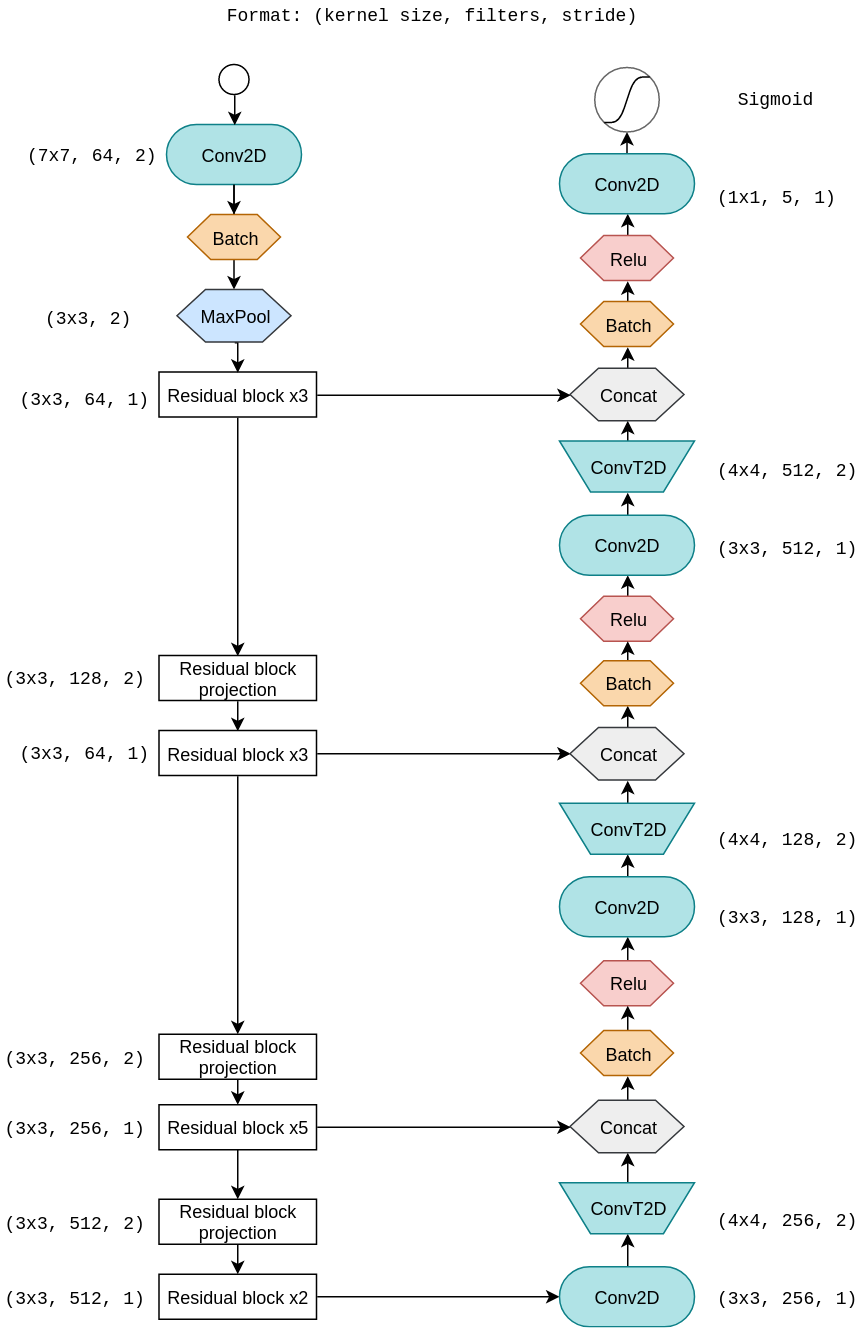
\includegraphics[width=0.45\textwidth]{architectures/detector.png}
	\label{fig:detector}
\end{figure}

\noindent During the encoding phase, the input image of dimension $512 \times 512$ is shrunk through 5 convolutional blocks.\\
The first block uses a convolution of size 7 and stride 2 and a max pooling operation to downsample the image by a factor of 4.\\
The second block is built of 3 standard residual blocks with identity shortcut. Such a block can be visualized in figure \ref{fig:resblock_1}. These blocks do not change the image dimension and they just apply two convolutions to add more feature maps, with the addition block at the end.\\
The third block halves the image size using a residual block with projection shortcut (in figure \ref{fig:resblock_2}) and three residual blocks with identity shortcut.\\
Fourth and fifth blocks just repeat this steps with a different number of identity shortcut blocks. Note that each residual block double the number of channels in the image. For what concerns the decoder, the encoded input of size $(16, 16, 512)$ is passed to the decoder that uses three up-convolutional blocks to upsample it to the desired output dimension of $(128, 128, 5)$. Here, we made two major changes with respect to the standard CenterNet implementation of the decoder:

\begin{enumerate}
	\item We added cross connections in U-Net fashion, and
	\item We replaced the deformable convolution layer with a simple convolution.
\end{enumerate}

\begin{figure}[h]
	\caption{Residual block with identity shortcut.}
	\centering
	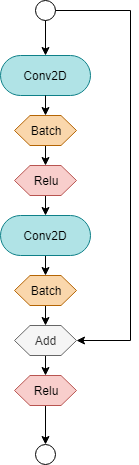
\includegraphics[width=0.1\textwidth]{architectures/resblock_1.png}
	\label{fig:resblock_1}
\end{figure}

\begin{figure}[h]
	\caption{Residual block with projection shortcut.}
	\centering
	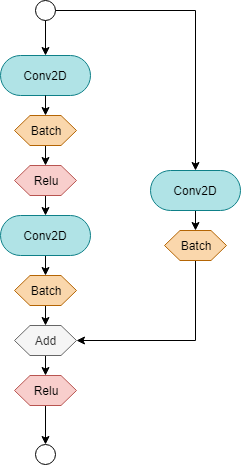
\includegraphics[width=0.2\textwidth]{architectures/resblock_2.png}
	\label{fig:resblock_2}
\end{figure}

The difference between a standard convolution and deformable convolution is that using the former the receptive field and the sampling locations are fixed all over the top feature map, while using the latter they are adaptively adjusted according to the scale and shape of the objects in deformable convolution. This is implemented by augmenting the standard convolutional grid with a matrix of parameters called offsets, which must be learned in addition to the standard convolution weights \cite{DeformableConv2017}. The authors of the original paper reported an improvement over standard convolution for object detection tasks, in particular in the detection of irregular objects. On the other hand, the characters to be recognised in the Kuzushiji documents are arranged in adjacent columns, in a grid-like pattern. For this reason, and considering the additional computational time required to train a deformable convolutional network, we decided to replace them with their standard counterparts. \\

The decoder is composed of three identical blocks, each featuring the following layers:

\begin{itemize}
	\item a convolution to reduce the number of features;
	\item a transposed convolution to upsample the image by a factor of 2;
	\item a concatenate operation that concatenates the output of a block of the encoder with the output of the transposed convolution;
	\item a batch normalization to reduce variances of values;
	\item a leaky ReLu activation.
\end{itemize}

The last block is composed of a $1 \times 1$ convolution to reduce the number of features to 5 and a sigmoid activation. The final output is an array with 3 dimensions shaped as $(128, 128, 5)$. This output is the predicted heatmap $\widehat{Y}$. Each of the five layers in the outer dimension has the same meaning explained above, with the difference that the “ground truth map” is not predicted, since this information is provided inside the heatmap itself. This is the reason why the output has 5 instead of 6 layers for each image.

\subsubsection{Pre-processing and training}
\label{sssec:preprocessingdet}

The input samples are firstly resized to $512 \times 512 \times 3$ and normalized, as well as random cropped for data augmentation. A maximum crop factor is determined considering the average character size in the page. This is determined separatedly for width and height as shown in equations \ref{eq:stretchw} and \ref{eq:stretchh}, where $w$ and $h$ are the dimensions of the original image and $char\_area$ is the average bounding box area within the page.
\begin{equation}\label{eq:stretchw}
	c_w=\sqrt{\frac{w \cdot h}{char\_area}}
\end{equation}
\begin{equation}
\label{eq:stretchh}
	c_h=\frac{h}{w}\sqrt{\frac{w \cdot h}{char\_area}}
\end{equation}
This crop procedure allows to train the network on smaller fragment of pages with better recognition rate of small sharacters. In addition, this step ensures good recognition performances when paired with the post-processing passage described in the next section.\\
\noindent Finally, all output classes, expressed as unicode characters, are mapped to integer values.

\subsubsection{Post-processing: from centers to bounding boxes}
\label{sssec:preprocessingandtraining}

The previously described network predicts the location of the center of each character within the page. From that we infer the coordinates of the bounding box location using the size information in the predicted heatmap ($Y_{x,y,3}$ and $Y_{x,y,4}$) and summing the offsets ($Y_{x,y,1}$ and $Y_{x,y,2}$). To further improve the accuracy of the bounding boxes, some post-processing has been made as well. Firstly, all heatmap elements with score prediction below 0.7 were filtered out, since they probably represent noise. The remaining ones are the predicted centers. The predicted offsets are then added to the coordinates of these centers in the heatmap and the definitive coordinates of the bounding boxes are computed as:
\begin{eqnarray*}
	xmin=x_c - \frac{width}{2}\\
	ymin= y_c - \frac{height}{2}\\
	xmax=x_c + \frac{width}{2}\\
	ymax=y_c + \frac{height}{2}
\end{eqnarray*}
Then, out-of-picture boxes and the ones with an area too different from the average area in the page (too big or too small) are removed. Finally overlap-based non maximum suppression is performed comparing the intersection area between the boxes. Each lower score bounding box sharing more than 40\% of the area of higher score boxes, or having more than 60\% of its area inside other higher score bounding boxes is removed.\\

\noindent Despite the non-maximum-suppression, we noted that some small characters were not detected by the network. This happens because the feature map is, in some cases, too small with respect to the original image, and may lose some information, leading to lower IoU score with the ground truth bounding boxes. 
Our solution was to divide each image into a number $n$ of smaller images (that we call \textit{tiles}) and use the model to predict bounding boxes in each one of the smaller images. A 25\% overlap between the tiles is used to preserve the objects along the tile boundaries and prevent any miss due to image partitioning. An example of partitioned image is shown in figure \ref{fig:tiles4}.

\begin{figure}
	\centering
	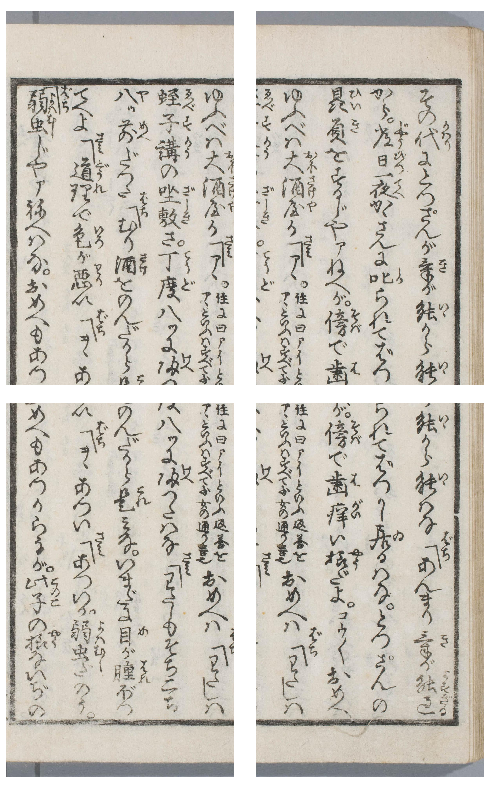
\includegraphics[width=0.8\columnwidth]{detection/tiles_4.png}
	\caption{An image divided in 4 tiles with 25\% overlapping}
	\label{fig:tiles4}
\end{figure}

This procedure resulted in more precise bounding box predictions and an higher IoU score on the test set. A comparison can be seen in figure \ref{fig:comparisontiling}. \\
We empirically determined the optimal number of tiles by measuring the IoU score over the same first 100 examples of the test set. Results gave a 0.7731 score using a $2 \times 2$ grid and 0.7850 using a $3 \times 3$ grid. 
Since the difference in the IoU score was negligible we chose to use a $2 \times 2$ grid, with the benefit of halving the time required to generate predictions for a single image.\\
It's worth to say that the same model trained without the random crop described in §\ref{sssec:preprocessingdet} did not reach such scores, but rather got an average IoU score of 0.53. This probably means that the crop procedure enhances the ability of the model to detect small features, particularly useful when predicting portions of images.

\begin{figure*}[h!]
	\centering
	\begin{subfigure}{\columnwidth}
		\centering
		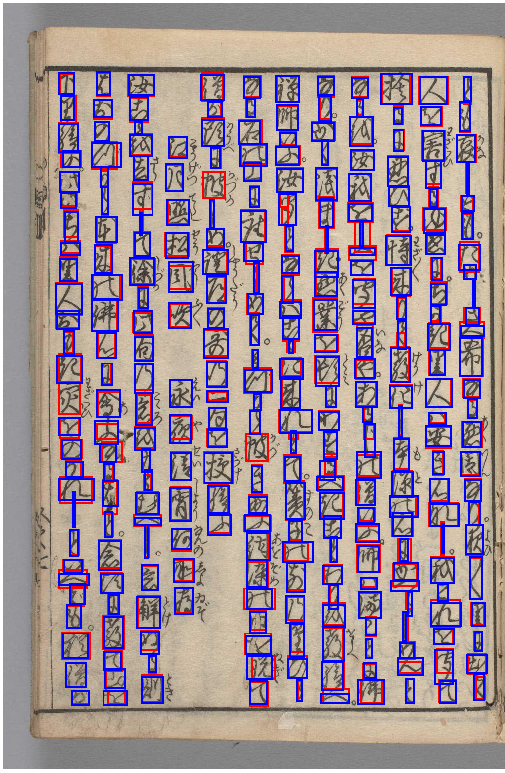
\includegraphics[width=0.9\columnwidth]{detection/tiled_prediction.png}
		\caption{Predicion with $2\times2$ tiling}
		\label{fig:tiledpred}
	\end{subfigure}
	\begin{subfigure}{\columnwidth}
		\centering
		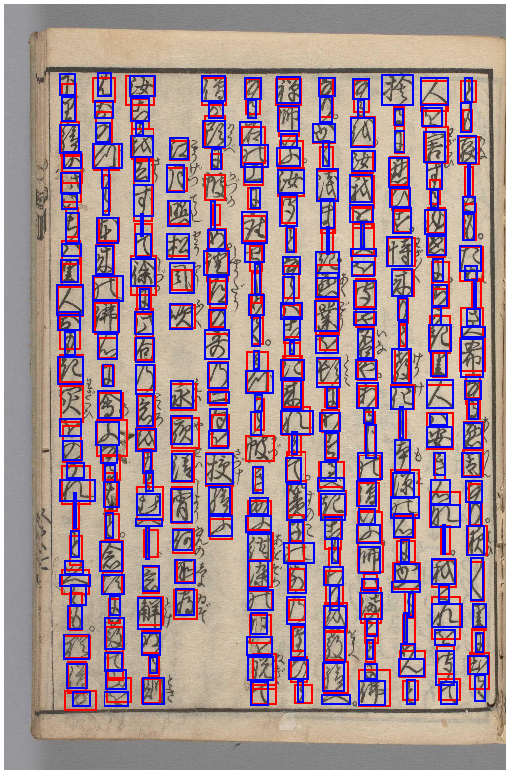
\includegraphics[width=0.91\columnwidth]{detection/standard_prediction.png}
		\caption{Predicion with no tiling}
		\label{fig:standardpred}
	\end{subfigure}
	\caption{Comparison of predicion on the same page with or without tiling. Image (\ref{fig:tiledpred}) has a IoU score of 0.83, while (\ref{fig:standardpred}) scored 0.59.}
	\label{fig:comparisontiling}
\end{figure*}

\subsection{Classification of characters using a standard CNN}
\label{ssec:classificationcnn}

While the model described in the previous section was used to detect characters, the goal of the classifier is to classify each detected character in one of the 4212 current Japanese characters, hopefully the one corresponding to its translation. The number of classes in our model is the number of different Kuzushiji characters found in the training set. In the official dataset for the competition, a dictionary of 4787 Kuzushiji characters and their translation was provided, but not all of them are present in the training set, while other characters are extremely rare. This may lead to worse classification performances for characters the model has seen fewer times.

\subsubsection{Implementation}
\label{sssec:implementationclass}

\subsubsubsection{Network architecture}
\label{ssssec:networkarchitectureclass}

The classifier is a small convolutional model based on the one proposed in the Kaggle implementation. The architecture diagram is shown in figure \ref{fig:classifier}. The three repeated blocks are followed by an average pooling layer with kernel size equal to the input dimension (named global pooling), which produce a single value for each feature map. This value is then fed to the final dense layer with softmax activation and number of units equal to the number of categories. We tested some simple variations using different types of residual blocks, and they worked equally well, so we didn not spend much time experimenting with other architectures.

\begin{figure}[h]
	\caption{Architecture of the classifier.}
	\centering
	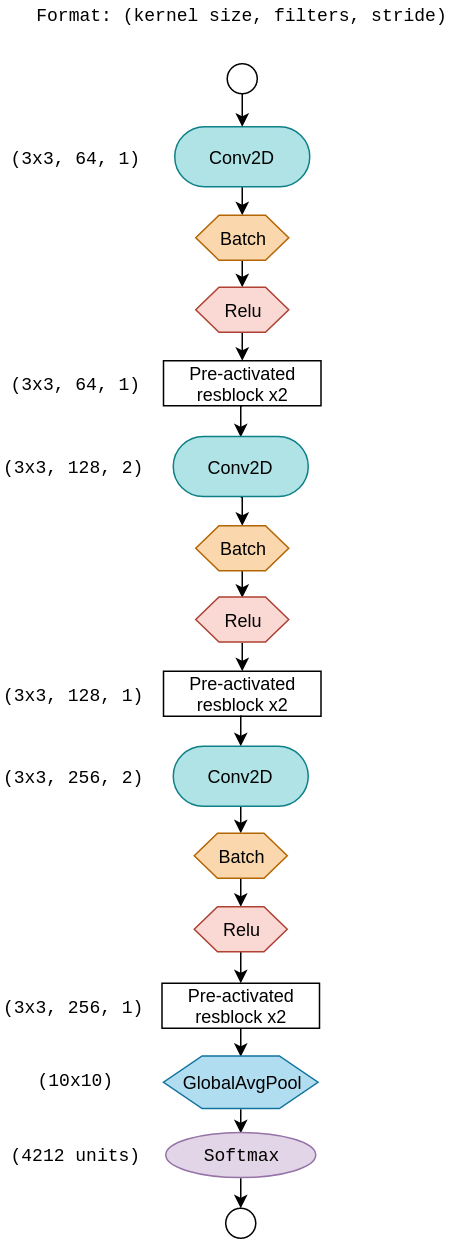
\includegraphics[width=0.25\textwidth]{architectures/classifier.png}
	\label{fig:classifier}
\end{figure}

\subsubsubsection{Loss function}
\label{ssssec:lossfunctionclass}

Since the character classes are codified as integers, we used sparse categorical crossentropy to evaluate the error of the model. 

\subsubsection{Pre-processing and training}
\label{sssec:preprocessingclass}

In order to deal with the main challenging features of cursive handwritten text, some data augmentation has been made on the $32 \times 32$ cropped and resized images of the detected characters. In particular, the objective was emulating the imprecision, variability and deformation inherent the writing of the characters. For this purpose, the dataset has been augmented with copies of the original images slightly altered with respect to brightness, rotation, width and height shifts, and zoom. The augmentation has been performed using the \textit{ImageDataGenerator} utility provided by Keras. 
We trained the classification network with 'Adam' optimizer, configured with Keras default hyperparameters, with batch size 1024 and using a learning rate of $1 \cdot 10-5$.

% --- EXPERIMENTS ---

%\clearpage
% !TeX spellcheck = en_US
\section{EXPERIMENTS}
\label{sec:experiments}

For the sake of comparing the results of the experiments, we divided the Kaggle training set into a test and validation set (15\% of the whole dataset each) leaving the remaining 70\% of the examples for training. We then split the dataset for the classifier, consisting in the totality of the cropped detected characters, in the same way. The examples within the test set remain the same through each execution, and the loss and accuracy metrics reported further on are computed with respect to the test set. We list the metrics for the two models separately, adding the overall Kaggle rating received over submission of the predictions for the whole test set. Submissions to the competition are evaluated on a modified version of the F1 Score. To score a true positive, center point coordinates that are within the ground truth bounding box and a matching label must be provided. We used the ResNet34-encoded model for the final submission, since it was the one yielding the best results.

\subsection{Detector}
\label{ssec:detectorexp}

All models were trained using Adam optimizer using the default Keras hyper-parameters for 130 epochs. For the ResNet34 network we used a learning rate of $1 \cdot 10^{-4}$ for the first 10 epochs, decreasing it to $5 \cdot 10^{-5}$ for the next 50 epochs and using $1 \cdot 10^{-5}$ for the last 70 epochs. We used a single GPU Tesla T4 provided by Google Cloud Platform with batch size 32.\\
The same values were used for pretrained ResNet50 network except for batch size, that we set to 16 because of the deeper architecture, and for learning rate that we further lowered to $5 \cdot 10^{-6}$ after 50 epochs, since the loss function was not converging. Subsequent experiments restarting the training with lower learning rates did not improve the results. The results of the experiments are summarized in \ref{tab:detec-res}

\begin{table*}[h]
	\begin{tabular}{lllllll}
		\rowcolor[HTML]{EFEFEF} 
		\textbf{Experiment}   & \textbf{Loss} & \textbf{Heatmap loss} & \textbf{Offset loss} & \textbf{Size loss} & \textbf{IoU (no tiling)} & \textbf{IoU (tiling)} \\
		ResNet34 encoder      & 1.2652        & 0.7887                & 0.3833               & 0.0932             & 0.5112                   & 0.7658                \\
		ResNet50 encoder      & 1.3792        & 0.8417                & 0.4092               & 0.1284             & 0.4067                   & 0.6659                   
	\end{tabular}
	\label{tab:detec-res}
\end{table*}

\subsection{Classifier}
\label{ssec:classifierexp}

The classifier was trained using Adam optimizer and learning rate $5 \cdot 10^{-4}$ for the first 4 epochs, $1 \cdot 10^{-4}$ for the next 2 epochs, and $5 \cdot 10^{-5}$ for the following ones. The value of the learning rate was decreased manually when we noted oscillations in the validation loss value. In table \ref{tab:class-res} are reported two experiments. The first model used an alternative architecture using standard residual blocks as depicted in fig \ref{fig:resblock_1} and was trained without data augmentation. The second one had the architecture described in \ref{fig:preact_resblock} with preactivated residual blocks and was trained using data augmentation. The final submission has been done only using this last model.

\begin{table*}[h]
	\begin{tabular}{llll}
		\rowcolor[HTML]{EFEFEF} 
		\textbf{Experiment} & \textbf{Loss} & \textbf{Accuracy} & \textbf{Kaggle score with ResNet34} \\
		Residual block 1    &               &                   &                                     \\
		Residual block 2    &               &                   &                                    
	\end{tabular}
	\label{tab:class-res}
\end{table*}

\begin{figure}[h]
	\caption{Preactivated residual block.}
	\centering
	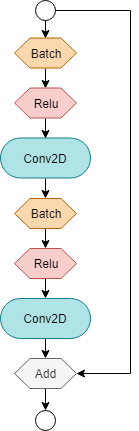
\includegraphics[width=0.15\textwidth]{architectures/preactivated_resblock.png}
	\label{fig:preact_resblock}
\end{figure}

\section{Benchmarks related to similar results}
\label{sec:stateofart}

\subsection{Handwritten text recognition on historical documents}
\label{ssec:historicaldocuments}

\cite{Sanchez2019-pi} introduces four HTR (Handwritten Text Recognition) benchmarks aimed at HTR research for historical and legacy documents. These benchmarks are based on the datasets and rules previously adopted in well known open HTR competitions. The first two of these competitions (datasets ICFHR-2014, ICDAR-2015) were based on parts of the so called Bentham Papers, handwritten in English by several writers. The whole digitized collection encompasses 100000 page images of text authored by the renowned English philosopher and reformer Jeremy Bentham (1748–1832). It mainly contains legal forms and drafts in English, but also some pages are in French and Latin. Many images entail important pre-processing and layout analysis difficulties, like marginal notes, faint ink, stamps, skewed images, lines with large slope variation within the same page, slanted script, inter-line text, etc. An example of these documents is shown in figure \ref{fig:HTR_benchmark}.

\begin{figure}[h]
	\caption{An example of image from the Bentham Papers.}
	\centering
	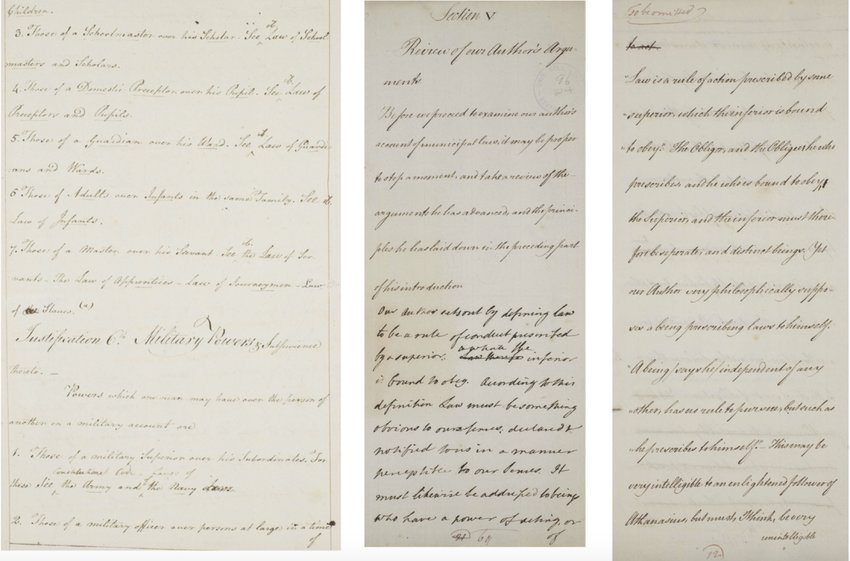
\includegraphics[width=0.45\textwidth]{various/HTR_benchmark.png}
	\label{fig:HTR_benchmark}
\end{figure}

In the third competition, the Ratsprotokolle collection (ICFHR-2016), composed of handwritten minutes of council meetings held from 1470 to 1805, was considered, while the dataset of the fourth competition was a part of the Alfred Escher Letter Collection (AEC, ICDAR-2017) which is composed of letters handwritten mainly in German but it also has pages in French and Italian. Table \ref{tab:htr-benchmarks} summaries the baselines achieved by \cite{Sanchez2019-pi} and the best results achieved prior the publication of their paper. Note that the Word Error Rate (WER) and the Character Error Rate (CER) metrics are used. WER is defined as the minimum number of words that need to be substituted, deleted, or inserted to match the recognition output with the corresponding reference ground truth, divided by the total number of words in the reference transcripts. CER is defined in the same way but at character level.

\begin{table*}[h]
	\begin{tabular}{ccccc}
		\rowcolor[HTML]{EFEFEF} 
		\cellcolor[HTML]{EFEFEF}                                     & \multicolumn{2}{l}{\cellcolor[HTML]{EFEFEF}\textbf{Best so far}} & \multicolumn{2}{l}{\cellcolor[HTML]{EFEFEF}\textbf{HTR benchmarks paper}} \\
		\rowcolor[HTML]{EFEFEF} 
		\multirow{-2}{*}{\cellcolor[HTML]{EFEFEF}\textbf{Benchmark}} & CER(\%)                         & WER(\%)                        & CER(\%)                             & WER(\%)                             \\
		ICFHR-2014 Restricted                                        & 5.0                             & 14.6                           & 5.0                                 & 9.7                                 \\
		ICDAR-2015 Restricted                                        & 15.5                            & 30.2                           & 12.8                                & 30.0                                \\
		ICFHR-2016 Restricted                                        & 4.8                             & 20.9                           & 4.5                                 & 17.5                                \\
		ICDAR-2017 Traditional                                       & 7.0                             & 19.1                           & 5.8                                 & 17.6                                \\
		ICDAR-2017 Advanced                                          & 6.4                             & 16.8                           & 6.3                                 & 18.5                               
	\end{tabular}
	\label{tab:htr-benchmarks}
\end{table*}

\subsection{Image classification on Kuzushiji-MNIST}
\label{ssec:imagemnist}

MNIST, a dataset with 70,000 labeled images of handwritten digits, has been one of the most popular datasets for image processing and classification for over twenty years. Despite its popularity, contemporary deep learning algorithms handle it easily, often surpassing an accuracy result of 99.5\%. Kuzushiji-MNIST \cite{Clanuwat2018-vm} is an alternative dataset to MNIST, more difficult than MNIST. The Kuzushiji dataset includes characters in both Kanji and Hiranaga, based on pre-processed images of characters from 35 books from the 18th century. It is constituted by three groups of data, as shown in table \ref{tab:kuzushiji-struct}. The creators of the Kuzushiji-MNIST dataset created a baseline by training a few classification algorithms and comparing them to MNIST. The best algorithm (PreActResNet-18) achieved 99.56\% on MNIST, but only 98.83\% and 97.33\% accuracy on Kuzushiji-MNIST and Kuzushiji-49 respectively, as can be seen in table \ref{tab:kuzushiji-benchmarks}.

\begin{table*}[h]
	\begin{tabular}{lllll}
		\rowcolor[HTML]{EFEFEF} 
		\textbf{Dataset} & \textbf{Classes}       & \textbf{Dataset Size} & \textbf{Balanced Classes} & \textbf{Image Size} \\
		Kuzushiji-MNIST  & 10 Hiragana characters & 70.000                & Yes                       & 28x28               \\
		Kuzushiji-49     & 49 Hiragana characters & 270.912               & No                        & 28x28               \\
		Kuzushiji-Kanji  & 3832 Kanji characters  & 140.426               & No                        & 64x64              
	\end{tabular}
	\label{tab:kuzushiji-struct}
\end{table*}

\begin{table*}[h]
	\begin{tabular}{lccc}
		\rowcolor[HTML]{EFEFEF} 
		\textbf{Model}                            & \textbf{MNIST {[}16{]}} & \textbf{Kuzushiji-MNIST} & \textbf{Kuzushiji-49} \\
		4-Nearest Neighbour Baseline              & 97.14\%                 & 91.56\%                  & 86.01                 \\
		Keras Simple CNN Benchmark {[}4{]}        & 99.06\%                 & 95.12\%                  & 89.25\%               \\
		PreActResNet-18 {[}11{]}                  & \textbf{99.56\%}        & 97.82\%                  & 96.64\%               \\
		PreActResNet-18 + Input Mixup {[}26{]}    & 99.54\%                 & 98.41\%                  & 97.04\%               \\
		PreActResNet-18 + Manifold Mixup {[}22{]} & 99.54\%                 & \textbf{98.83\%}         & \textbf{97.33\%}     
	\end{tabular}
	\label{tab:kuzushiji-benchmarks}
\end{table*}

% --- CONCLUSION ---

% !TeX spellcheck = en_US
\section{CONCLUSIONS}
\label{sec:conclusions}

The objective of the project was accurately recognizing handwritten cursive Kuzushiji characters in ancient historical documents, which has been accomplished via a region-based object recognition approach. The illustrated model featured a CenterNet like detector followed by a CNN classifier, and achieved satisfying performances.\\

We concluded the competition with a sensible overall Kaggle score of \textcolor{red}{SCORE}. However, many improvements could have been tested. For example, a more tailored tiling and preprocessing would have probably resulted in a better accuracy of the predictions. Furthermore it could have been worth to try different encoding and decoding architectures for the detection model, like VGG and Hourglass, which are also referenced in the CenterNet paper. Using a totally different approach, Mask R-CNN could have been used to detect the characters, since it can generate a pixel-wise mask that seems suitable to recognize characters shapes. The usage of a recurrent model to add context information on each character classification, could have resulted in an improvement as well. Like reported on the dataset description of the competition, indeed, some Kuzushiji characters are very similar, differing just for small details, and their meaning can be more easily inferred from context than by looking at the single character itself.


% -- BENCHMARKS ---

%\clearpage
\appendix
% !TeX spellcheck = en_US
\section{\uppercase{Benchmarks and similar results}}
\label{sec:stateofart}

\subsection{Handwritten text recognition on historical documents}
\label{ssec:historicaldocuments}

\citeauthor{Sanchez2019-pi}\cite{Sanchez2019-pi} introduces four HTR (Handwritten Text Recognition) benchmarks aimed at HTR research for historical and legacy documents. These benchmarks are based on the datasets and rules previously adopted in well known open HTR competitions. The first two of these competitions (datasets ICFHR-2014, ICDAR-2015) were based on parts of the so called Bentham Papers, handwritten in English by several writers. The whole digitized collection encompasses 100000 page images of text authored by the renowned English philosopher and reformer Jeremy Bentham (1748–1832). It mainly contains legal forms and drafts in English, but also some pages are in French and Latin. Many images entail important pre-processing and layout analysis difficulties, like marginal notes, faint ink, stamps, skewed images, lines with large slope variation within the same page, slanted script, inter-line text, etc. An example of these documents is shown in figure \ref{fig:HTRbenchmark}.

\begin{figure}[htb]
	\caption{An example of image from the Bentham Papers.}
	\centering
	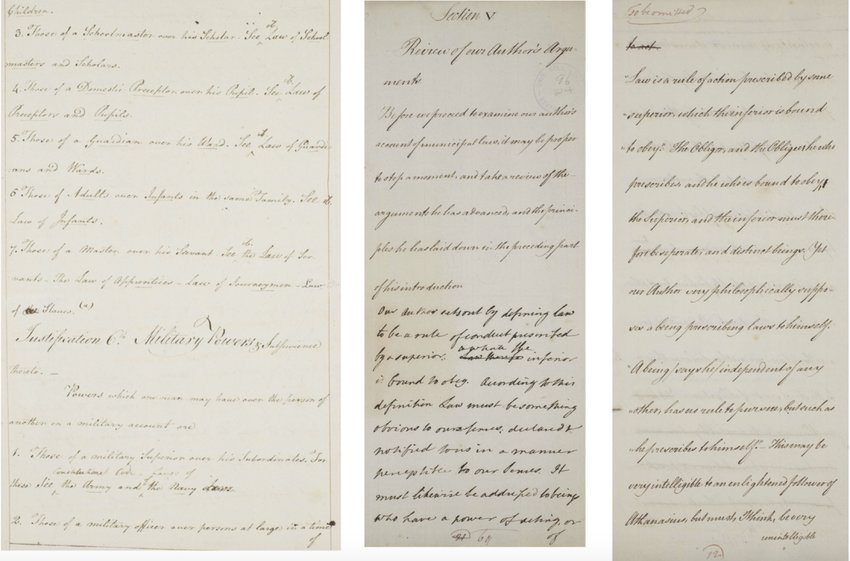
\includegraphics[width=0.45\textwidth]{various/HTR_benchmark.png}
	\label{fig:HTRbenchmark}
\end{figure}

In the third competition, the Ratsprotokolle collection (ICFHR-2016), composed of handwritten minutes of council meetings held from 1470 to 1805, was considered, while the dataset of the fourth competition was a part of the Alfred Escher Letter Collection (AEC, ICDAR-2017) which is composed of letters handwritten mainly in German but it also has pages in French and Italian. Table \ref{tab:htr-benchmarks} summarizes the baselines achieved by \cite{Sanchez2019-pi} and the best results achieved prior the publication of their paper. Note that the Word Error Rate (WER) and the Character Error Rate (CER) metrics are used. WER is defined as the minimum number of words that need to be substituted, deleted, or inserted to match the recognition output with the corresponding reference ground truth, divided by the total number of words in the reference transcripts. CER is defined in the same way but at character level.

\begin{table*}
	\begin{tabular}{lcccc}
		\rowcolor[HTML]{EFEFEF}
		\cellcolor[HTML]{EFEFEF}                                     & \multicolumn{2}{l}{\cellcolor[HTML]{EFEFEF}\textbf{Best so far}} & \multicolumn{2}{l}{\cellcolor[HTML]{EFEFEF}\textbf{HTR benchmarks paper}} \\
		\rowcolor[HTML]{EFEFEF}
		\multirow{-2}{*}{\cellcolor[HTML]{EFEFEF}\textbf{Benchmark}} & CER(\%)                         & WER(\%)                        & CER(\%)                             & WER(\%)                             \\
		ICFHR-2014 Restricted                                        & 5.0                             & 14.6                           & 5.0                                 & 9.7                                 \\
		ICDAR-2015 Restricted                                        & 15.5                            & 30.2                           & 12.8                                & 30.0                                \\
		ICFHR-2016 Restricted                                        & 4.8                             & 20.9                           & 4.5                                 & 17.5                                \\
		ICDAR-2017 Traditional                                       & 7.0                             & 19.1                           & 5.8                                 & 17.6                                \\
		ICDAR-2017 Advanced                                          & 6.4                             & 16.8                           & 6.3                                 & 18.5
	\end{tabular}
	\caption{Benchmarks on handwritten text recognition from \cite{Sanchez2019-pi}.}
	\label{tab:htr-benchmarks}
\end{table*}

\subsection{Image classification on Kuzushiji-MNIST}
\label{ssec:imagemnist}

MNIST, a dataset with 70,000 labeled images of handwritten digits, has been one of the most popular datasets for image processing and classification for over twenty years. Despite its popularity, contemporary deep learning algorithms handle it easily, often surpassing an accuracy result of 99.5\%. Kuzushiji-MNIST \cite{Clanuwat2018-vm} is an alternative dataset to MNIST, more difficult than MNIST. The Kuzushiji dataset includes characters in both Kanji and Hiranaga, based on pre-processed images of characters from 35 books from the 18th century. It is constituted by three groups of data, as shown in table \ref{tab:kuzushiji-struct}. The creators of the Kuzushiji-MNIST dataset created a baseline by training a few classification algorithms and comparing them to MNIST. The best algorithm (PreActResNet-18) achieved 99.56\% on MNIST, but only 98.83\% and 97.33\% accuracy on Kuzushiji-MNIST and Kuzushiji-49 respectively, as can be seen in table \ref{tab:kuzushiji-benchmarks}.

\begin{table*}
	\begin{tabular}{llccc}
		\rowcolor[HTML]{EFEFEF}
		\textbf{Dataset} & \textbf{Classes}       & \textbf{Dataset Size} & \textbf{Balanced Classes} & \textbf{Image Size} \\
		Kuzushiji-MNIST  & 10 Hiragana characters & 70.000                & Yes                       & 28x28               \\
		Kuzushiji-49     & 49 Hiragana characters & 270.912               & No                        & 28x28               \\
		Kuzushiji-Kanji  & 3832 Kanji characters  & 140.426               & No                        & 64x64
	\end{tabular}
	\caption{Description of the structure of the Kuzushiji-MNIST dataset from \cite{Clanuwat2018-vm}.}
	\label{tab:kuzushiji-struct}
\end{table*}

\begin{table*}
	\begin{tabular}{lccc}
		\rowcolor[HTML]{EFEFEF}
		\textbf{Model}                            & \textbf{MNIST {[}16{]}} & \textbf{Kuzushiji-MNIST} & \textbf{Kuzushiji-49} \\
		4-Nearest Neighbour Baseline              & 97.14\%                 & 91.56\%                  & 86.01                 \\
		Keras Simple CNN Benchmark {[}4{]}        & 99.06\%                 & 95.12\%                  & 89.25\%               \\
		PreActResNet-18 {[}11{]}                  & \textbf{99.56\%}        & 97.82\%                  & 96.64\%               \\
		PreActResNet-18 + Input Mixup {[}26{]}    & 99.54\%                 & 98.41\%                  & 97.04\%               \\
		PreActResNet-18 + Manifold Mixup {[}22{]} & 99.54\%                 & \textbf{98.83\%}         & \textbf{97.33\%}
	\end{tabular}
	\caption{Benchmarks on the Kuzushiji-MNIST dataset from \cite{Clanuwat2018-vm}.}
	\label{tab:kuzushiji-benchmarks}
\end{table*}

% --- BIBLIOGRAPHY ---

%\clearpage
\newpage
\printbibliography[title=REFERENCES]

\end{document}
